\subsection{Detalles de la actividad}
Capturas de pantalla donde se realizo las pruebas de seguridad evidencias de las rutas protegias acceso no autorizado.


\begin{figure}[!htb] 
    \centering 
    \caption{Pruebas en postman con tokens} 
    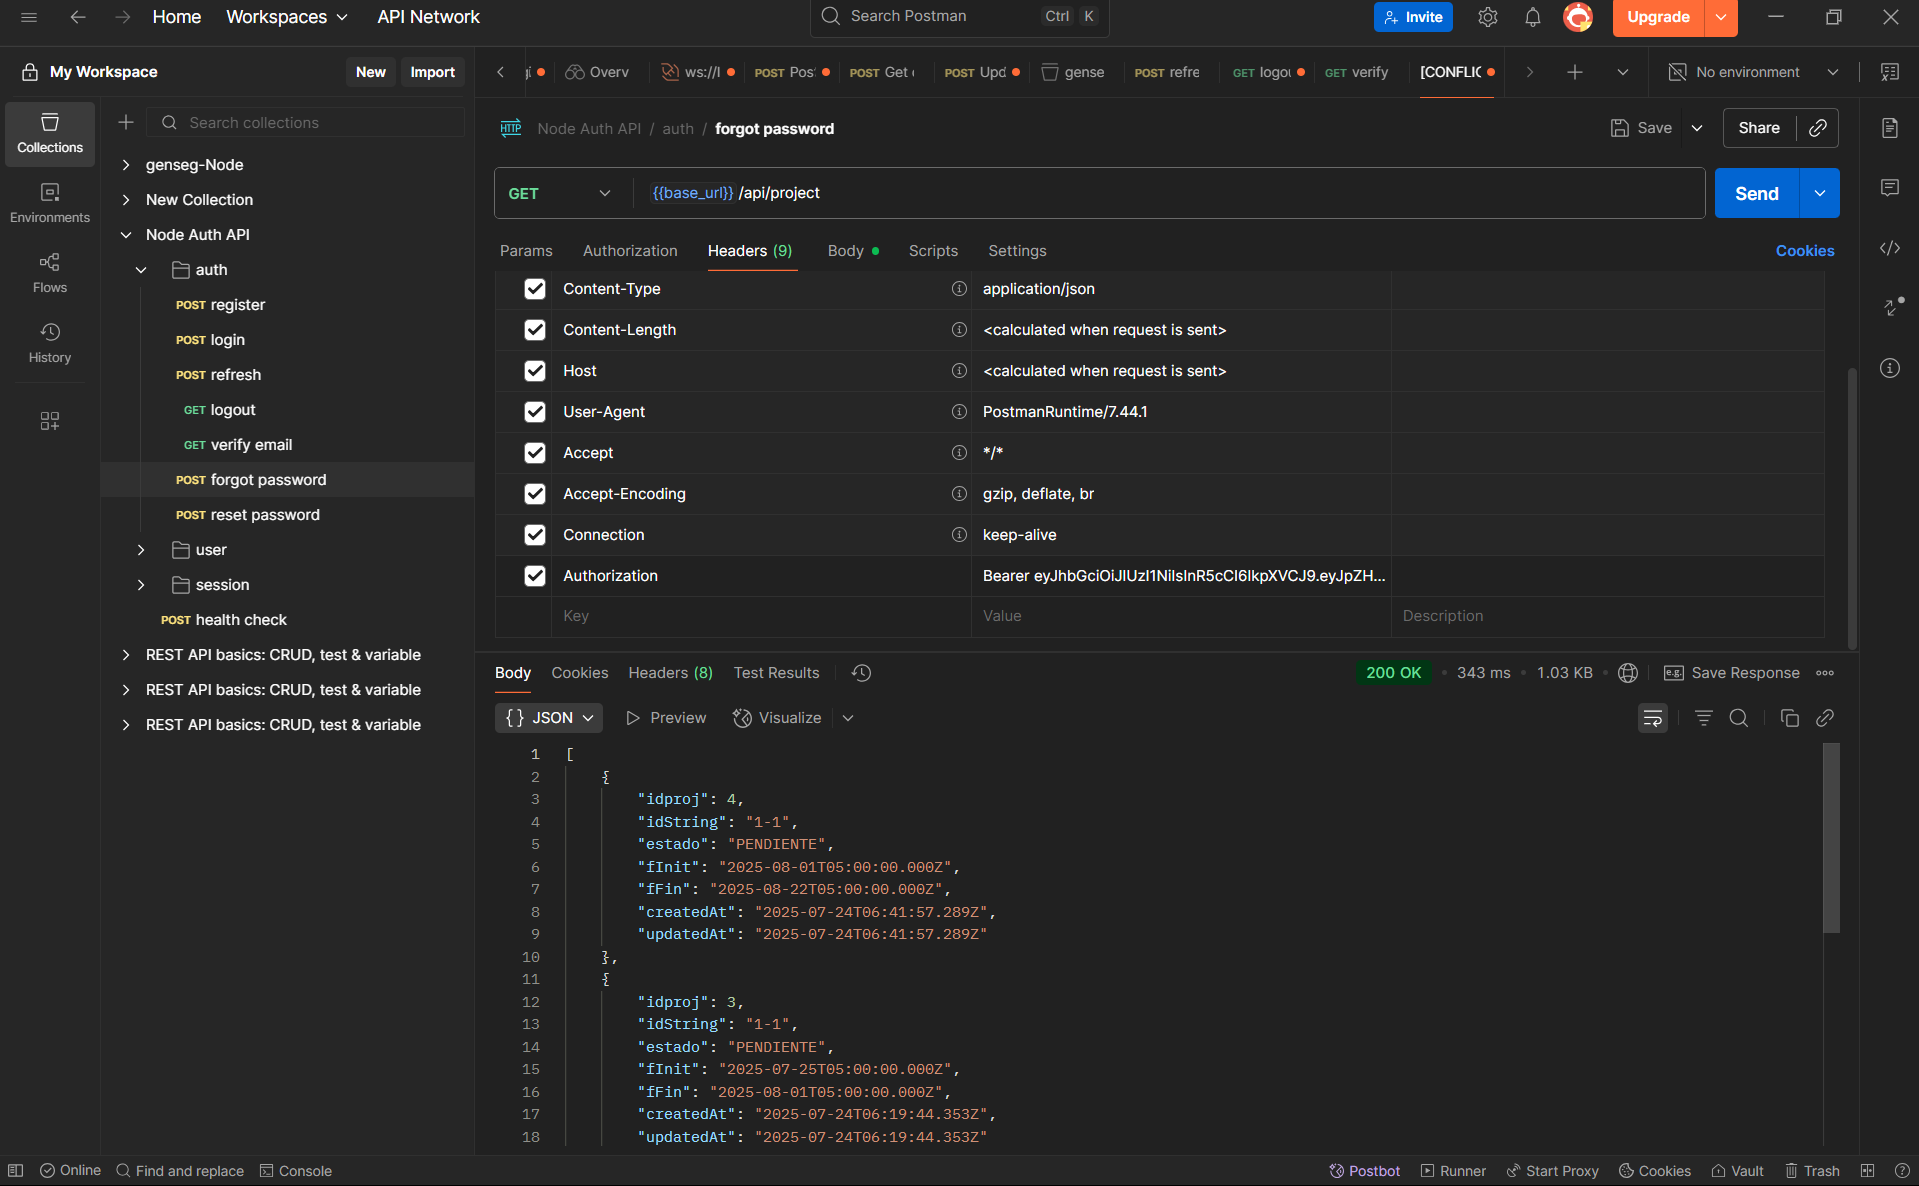
\includegraphics[width=0.8\textwidth]{images/postman.png} 
    \label{fig:postman} 
\end{figure} 
\FloatBarrier


\begin{figure}[!htb] 
    \centering 
    \caption{Pruebas de postman con acceso no autorizado} 
    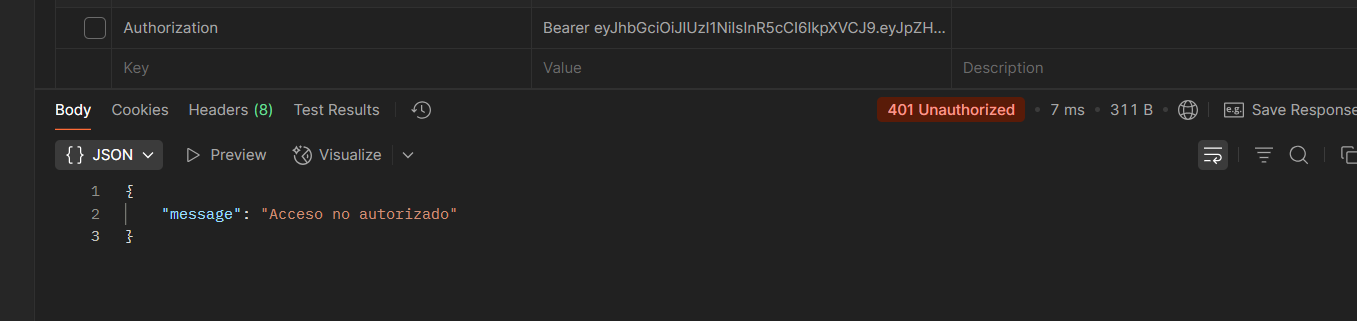
\includegraphics[width=0.8\textwidth]{images/postman1.png} 
    \label{fig:postman1} 
\end{figure} 
\FloatBarrier

\begin{figure}[!htb] 
    \centering 
    \caption{Pruebas de la API protegida} 
    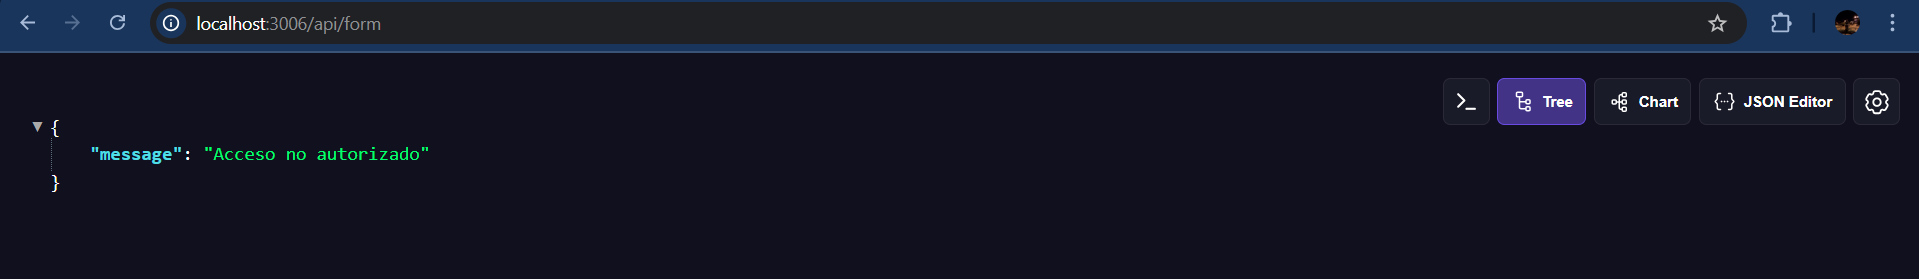
\includegraphics[width=0.8\textwidth]{images/api.png} 
    \label{fig:api} 
\end{figure} 
\FloatBarrier

\begin{figure}[!htb] 
    \centering 
    \caption{Base de datos en DB Bearer CE } 
    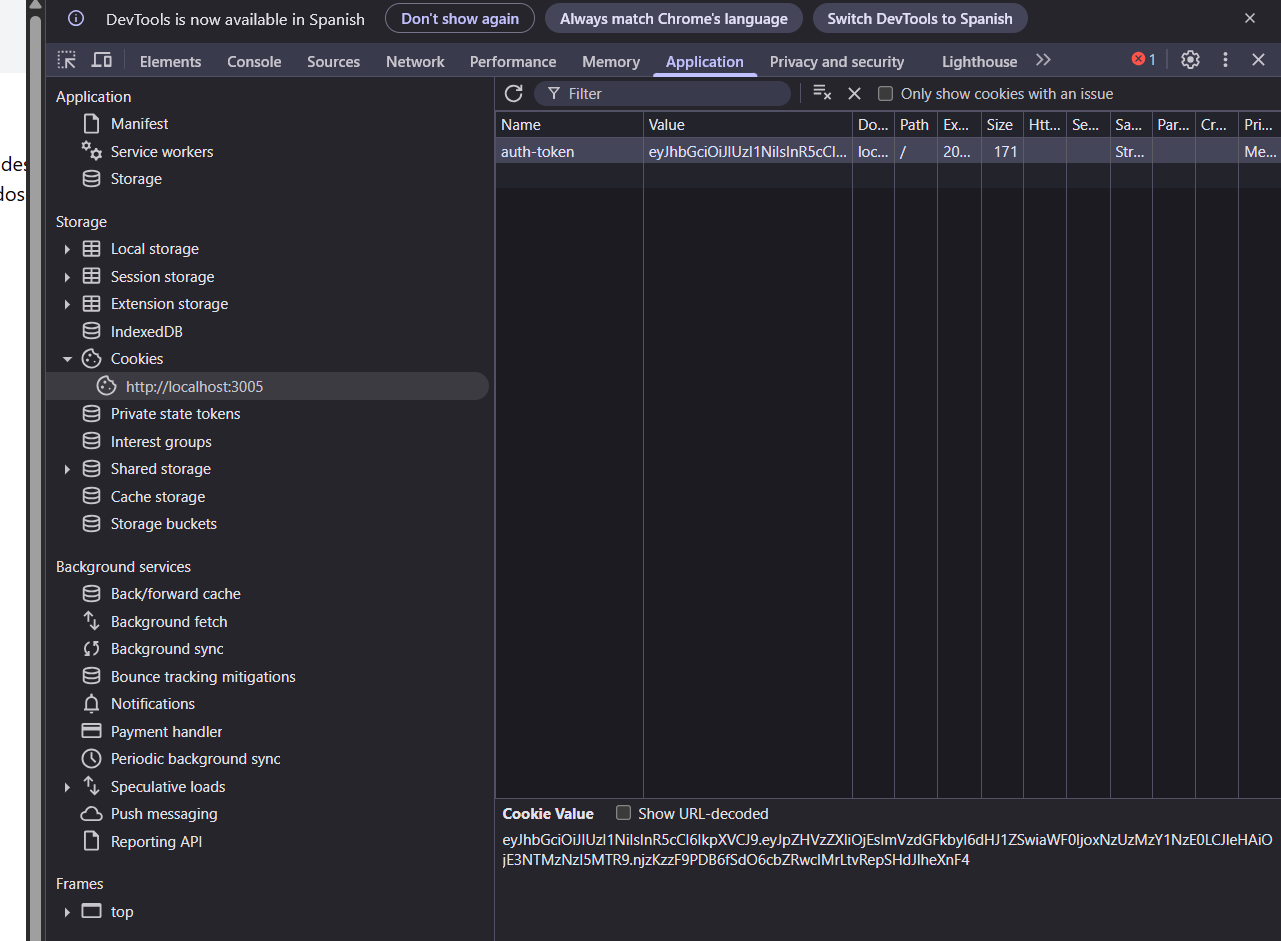
\includegraphics[width=0.8\textwidth]{images/bd.png} 
    \label{fig:db} 
\end{figure} 
\FloatBarrier

\begin{figure}[!htb] 
    \centering 
    \caption{Diagrama de la base de datos} 
    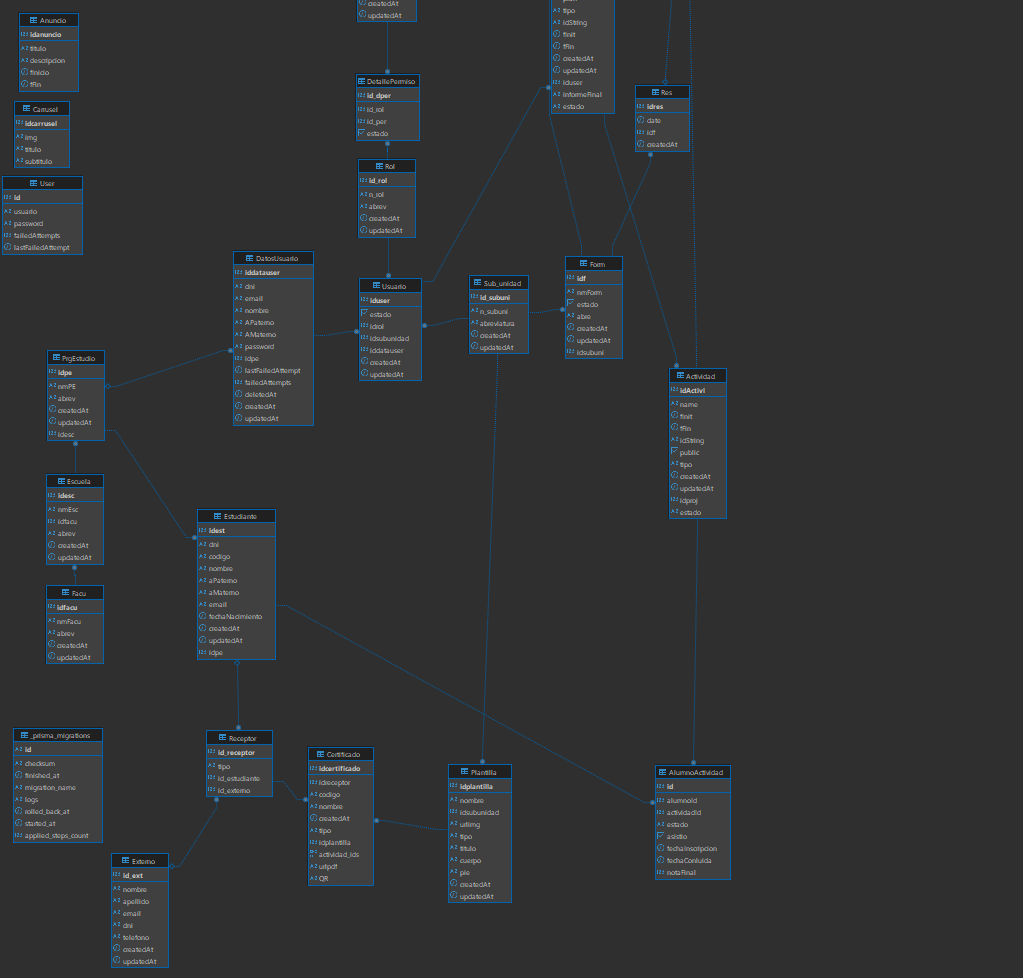
\includegraphics[width=0.8\textwidth]{images/diagrama.png} 
    \label{fig:diagrama} 
\end{figure} 
\FloatBarrier

\begin{figure}[!htb] 
    \centering 
    \caption{Verificacion de cifrado} 
    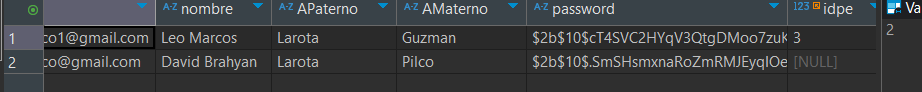
\includegraphics[width=0.8\textwidth]{images/cifrado.png} 
    \label{fig:cifrado} 
\end{figure} 
\FloatBarrier